% Copyright (c) 2014,2016 Casper Ti. Vector
% Public domain.

\chapter{技术二}\label{chapter:tal}

\section{算法示例}

算法~\ref{Algorithm:Chaining}中,如果一个结点$x$有一条标记为右括号的入边,另一个结点$y$有一条标记为左括号的出边,$x$到$y$存在一条路径,且这条路径上所有边的标记均为$e$,那么可以标记$y$为链结点。

\begin{algorithm} [ht]
\For {$x$是$G$的结点 $\wedge$ $x$至少有一条标记为右括号的入边} {
将$x$加入$C$; 将$x$加入$W$;
}
\While {$W$非空}{

取出并移除$W$的首个元素(记为$\varpi$);

\For {标记为$e$的$\varpi$的出边(记为$oe$)}{
将$oe$的标记变为右括号;\\
设$oe$将$\varpi$连结到$y$;\\
\If {$y\notin C$}{
将$y$加入$C$; 将$y$加入$W$;
}
}
}
\For {$y$是$G$的结点}{
\If {$y$至少有一条标记为右括号的入边 $\wedge$ $y$至少有一条标记为左括号的出边}{
将$y$标记为链结点;
}
}
\caption{识别链结点}
\label{Algorithm:Chaining}
\end{algorithm}

\section{图示例}

\textit{边界点.}
因为应用代码和摘要之间可达关系需要通过边界点进行传递,所以本文将所有\textit{边界点}作为关键摘要点。图\ref{fig:BoundaryNodes}\footnote{研究生院要求图标题放在图的后面。}展示了TALCRA摘要的四类边界点,其中的灰色结点表示摘要中的边界点,而白色表示应用代码结点。这四类结点的具体描述如下:
\begin{itemize}
\item 类型1边界点:如图\ref{fig:BoundaryNodes}(a)所示,应用代码通过库函数的调用将数值传给类型1边界点;
\item 类型2边界点:如图\ref{fig:BoundaryNodes}(b)所示,类型2边界点通过库函数的返回将数值传给应用代码;
\item 类型3边界点:如图\ref{fig:BoundaryNodes}(c)所示,类型3边界点通过回调函数的调用将数值传给应用代码;
\item 类型4边界点:如图\ref{fig:BoundaryNodes}(d)所示,应用代码通过回调函数的返回将数值传给类型4边界点。
\end{itemize}

\begin{figure}[htb]
\captionsetup[subfigure]{font=footnotesize}
\centering
\subcaptionbox{类型1边界点}[.25\textwidth]{%
	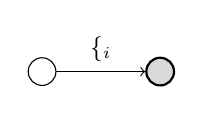
\begin{tikzpicture}[auto,->]
	\tikzstyle{cvertex}=[circle,draw=black,minimum size=10pt,inner sep=0pt]
	%\tikzstyle{cvertex}=[circle,draw=black,fill=white!15,minimum size=17pt,inner sep=0pt]
	\tikzstyle{lvertex}=[circle,fill=black!15,minimum size=10pt,inner sep=0pt]
	%\tikzstyle{lvertex}=[circle,fill=black!15,minimum size=17pt,inner sep=0pt]
	\tikzstyle{keyvertex}=[circle,thick,draw=black,fill=black!15,minimum size=10pt,inner sep=0pt]
	%\tikzstyle{keyvertex}=[circle,thick,draw=black,fill=black!15,minimum size=17pt,inner sep=0pt]
	\tikzstyle{weight} = [font=\small]
	\node[cvertex] (G-call) at (0,1.5) {};
	\node[keyvertex] (G-entry) at (1.5,1.5) {};
	\draw (G-call) -> node[weight] {$\{_i$} (G-entry);
	\end{tikzpicture}
}\label{fig:BoundaryNodes1}%
\subcaptionbox{类型2边界点}[.25\textwidth]{
	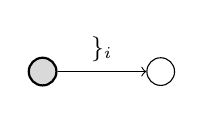
\begin{tikzpicture}[auto,->]
	\tikzstyle{cvertex}=[circle,draw=black,minimum size=10pt,inner sep=0pt]
	%\tikzstyle{cvertex}=[circle,draw=black,fill=white!15,minimum size=17pt,inner sep=0pt]
	\tikzstyle{lvertex}=[circle,fill=black!15,minimum size=10pt,inner sep=0pt]
	%\tikzstyle{lvertex}=[circle,fill=black!15,minimum size=17pt,inner sep=0pt]
	\tikzstyle{keyvertex}=[circle,thick,draw=black,fill=black!15,minimum size=10pt,inner sep=0pt]
	%\tikzstyle{keyvertex}=[circle,thick,draw=black,fill=black!15,minimum size=17pt,inner sep=0pt]
	\tikzstyle{weight} = [font=\small]
	\node[keyvertex] (G-exit) at (0,1.5) {};
	\node[cvertex] (G-return) at (1.5,1.5) {};
	\draw (G-exit) -> node[weight] {$\}_i$} (G-return);
	\end{tikzpicture}
}
\subcaptionbox{类型3边界点}[.25\textwidth]{%
	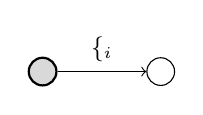
\begin{tikzpicture}[auto,->]
	\tikzstyle{cvertex}=[circle,draw=black,minimum size=10pt,inner sep=0pt]
	%\tikzstyle{cvertex}=[circle,draw=black,fill=white!15,minimum size=17pt,inner sep=0pt]
	\tikzstyle{lvertex}=[circle,fill=black!15,minimum size=10pt,inner sep=0pt]
	%\tikzstyle{lvertex}=[circle,fill=black!15,minimum size=17pt,inner sep=0pt]
	\tikzstyle{keyvertex}=[circle,thick,draw=black,fill=black!15,minimum size=10pt,inner sep=0pt]
	%\tikzstyle{keyvertex}=[circle,thick,draw=black,fill=black!15,minimum size=17pt,inner sep=0pt]
	\tikzstyle{weight} = [font=\small]
	\node[keyvertex] (G-call) at (0,1.5) {};
	\node[cvertex] (G-entry) at (1.5,1.5) {};
	\draw (G-call) -> node[weight] {$\{_i$} (G-entry);
	\end{tikzpicture}
}%
\subcaptionbox{类型4边界点}[.25\textwidth]{
	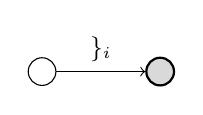
\begin{tikzpicture}[auto,->]
	\tikzstyle{cvertex}=[circle,draw=black,minimum size=10pt,inner sep=0pt]
	%\tikzstyle{cvertex}=[circle,draw=black,fill=white!15,minimum size=17pt,inner sep=0pt]
	\tikzstyle{lvertex}=[circle,fill=black!15,minimum size=10pt,inner sep=0pt]
	%\tikzstyle{lvertex}=[circle,fill=black!15,minimum size=17pt,inner sep=0pt]
	\tikzstyle{keyvertex}=[circle,thick,draw=black,fill=black!15,minimum size=10pt,inner sep=0pt]
	%\tikzstyle{keyvertex}=[circle,thick,draw=black,fill=black!15,minimum size=17pt,inner sep=0pt]
	\tikzstyle{weight} = [font=\small]
	\node[cvertex] (G-exit) at (0,1.5) {};
	\node[keyvertex] (G-return) at (1.5,1.5) {};
	\draw (G-exit) -> node[weight] {$\}_i$} (G-return);
	\end{tikzpicture}
}
\vspace{-2mm}
\caption{TALCRA摘要的四类边界点}\label{fig:BoundaryNodes}
%\vspace{-3mm}
\end{figure}

\section{表格示例}

表~\ref{tab:main}\footnote{研究生院要求表格标题放在表格前面。}展示了主要的实验结果。第2列是全程序的CFL分析实验效果。
第3到6列是应用代码分析的实验结果,第7到10列是构建库摘要的实验结果。

\begin{table}[h]
%\hspace{-10mm}
\center
\caption{\label{tab:main} 实验结果:TALCRA与CFLRA的运行时间和内存消耗对比}
\begin{tabular}{|c||r||rr|rr||rr|rr|}
\hline
程序&CFL&\multicolumn{4}{c||}{应用代码分析}&\multicolumn{4}{c|}{库代码摘要}\\\cline{3-10}
&&\multicolumn{2}{c|}{CFL}&\multicolumn{2}{c||}{TALCRA}&\multicolumn{2}{c|}{CFL}&\multicolumn{2}{c|}{TALCRA}\\
&总时间&时间&内存&时间&内存&时间&内存&时间&内存\\
&(ms)&(ms)&(MB)&(ms)&(MB)&(ms)&(MB)&(ms)&(MB)\\
\hline
\hline
check&615&348&152&67&58&267&107&645&132\\
compiler&639&330&153&53&73&309&130&661&141\\
compress&651&330&159&64&75&321&130&670&142\\
crypto&798&459&174&73&66&339&126&773&207\\
derby&1119&684&250&78&93&435&194&998&610\\
helloworld&592&309&130&36&48&283&105&640&138\\
mpegaudio&1622&1047&378&215&196&575&239&4421&387\\
scimark&653&331&161&67&78&322&131&665&149\\
startup&801&450&168&74&65&351&132&941&268\\
sunflow&583&290&123&33&44&293&100&663&127\\
xml&4378&2945&756&114&184&1433&587&5811&741\\
%\hline
%btree&105&80&48&56&179&68&264&155\\
%mushroom&80&64&8&48&169&76&183&93\\
%parser&108&86&13&53&199&74&269&158\\
%sample&61&64&13&48&162&73&184&99\\
\hline\hline
合计&12451&7523&&874&&4928&&16888&\\\hline
\end{tabular}
\end{table}

\section{代码示例}

图~\ref{fig:AbsClass}所示的上下文敏感数据依赖分析例子则表明,
库代码中的回调函数可能导致CFL可达性建立的库摘要产生漏报的情况。

\begin{figure}[htbp]
\begin{lstlisting}
package library;
public abstract class AbstractClass {
	public final int method1(int x1) {
		int y1 = x1 + 1;
		int z1 = method2(y1) + 1;
		return z1;
	}
	private final int method2(int x2) {
		int y2 = x2 + 2;
		int z2 = method3(y2) + 2;
		return z2;
	}
	abstract public int method3(int x3);
}
\end{lstlisting}
\caption{库代码示例}\label{fig:AbsClass}
\end{figure}

\section{其他环境示例}

其他环境包括定义、例子、定理、引理和证明。

\subsection{定义}

\begin{definition}[程序图]
程序图$G$是二元组$(V, E)$,其中$V$是结点集合,$E$是$V$中的结点之间的有向边的集合,每条边的标记是一个$\Sigma$中的符号。
\end{definition}

\subsection{例子}

\begin{example}
给定Datalog程序 $P = \langle \Sigma, \Gamma, I, O \rangle$,其中输入关系 $I = \{B,~C\}$, 输出关系 $O = \{D\}$。
\end{example}

\subsection{定理、引理和证明}

在证明序列的基础上给出关于规则实例化的引理\ref{lem:rule} 。

\newcommand{\vphi}[1]{\varphi_\mathbb{T}(#1)}
\newcommand{\rulesym}{::=}

\begin{lemma}\label{lem:rule} 
给定Datalog程序$P$、输入事实$D$和等价类抽象$\varphi_\mathbb{T}$,记适配后的程序为$P'$,$P$中的规则$\gamma$适配为规则$\gamma'$。
\end{lemma}

\begin{theorem}[正确性]\label{chap4:sound}
给定Datalog程序$P = \langle \Sigma, \Gamma, I, O \rangle$, 输入事实$D$, 等价类抽象$\varphi_\mathbb{T}$,对应元素到等价类的映射关系为$Abs$,适配后的程序为$P'$,则$P(D)$ $\subseteq$ $P'(D \cup Abs)$。
\end{theorem}
\begin{proof}
假设$w \in P(D)$,则存在证明序列$R^1_{0}(t^1_0), ..., R^i_{0}(t^i_0), ..., R^l_{0}(t^l_0)$%(引理\ref{datalogprove})
,使得
\begin{enumerate}
\item 
最后一个事实是 $w$, 即 $R^l_{0}(t^l_0) = w$;
\item 
序列中的每个事实属于$D$或由序列中前面的事实推理得来,即 
\[
R^i_{0}(t^i_0) ::= R^i_{1}(t^i_1), ..., R^i_{m^i}(t^i_{m^i}).
\]
\end{enumerate}

由$w$的任意性,$P(D) \subseteq P'(D \cup Abs)$。命题得证。

\end{proof}

\section{引用示例}

\textit{延迟式摘要}是一个与\textit{条件式摘要}相对应的概念\footnote{研究生院要求每一页的脚注都要从①标起。}。
近期大多数摘要技术都属于\textit{延迟式摘要}技术,例如构件级别分析CLA(Component Level Analysis)~\supercite{rountev2006interprocedural,DBLP:conf/cc/RountevSX08}、数据结构分析~\supercite{DBLP:conf/pldi/LattnerLA07}、模块化堆分析~\supercite{Madhaven2012modular}和Android框架的StubDroid技术~\supercite{BoddenICSE16}\footnote{研究生院要求按照引用的顺序对引文进行编号,并且用上角标标注引文编号}。

